Since the safety condition is a syntactic constraint, it can seem
difficult to give a characterization in term of game
semantics, as game models are by essence syntax-independent. This is where the the Correspondence Theorem comes to the rescue and help us to reason syntactically about the game denotation of a term. This ultimately permits us to give a precise game-semantic characterization of the safety restriction.

The main result of this chapter (Corollary
\ref{cor:safe_ptr_recoverable}) states that pointers in a play of
a strategy denoting  a safe term can be uniquely recovered
from O-questions' justification pointers and from the underlying sequence of
moves. We introduce the
notion of \emph{P-incrementally-justified strategies}, a particular kind of strategy in which justification pointers emanating from P-moves can be
reconstructed uniquely from the underlying sequences of moves and
from O-moves' pointers. We then introduce the notion of
\emph{incrementally-bound computation trees} and establish a relationship betwwen
incremental-binding and P-incremental-justification (proposition \ref{prop:Nher_incrbound_iff_incrjustified}). Finally, we show that safe simply-typed terms have incrementally\--bound computation trees, consequently their game denotation is P-incrementally-justified.


The first section of this chapter is concerned only with the safe $\lambda$-calculus without interpreted constants. In the next
section we extend the result by taking into account the interpreted
constants of \pcf\ and \ialgol. We define the language safe \ialgol\
(resp. safe \pcf) to be the fragment of \ialgol\ (resp. \pcf) where
the application and abstraction rules are constrained the same way
as in the safe $\lambda$-calculus. We show that safe \pcf\ terms are
denoted by P-incrementally-justified strategies and we give the key
elements for a possible extension of the result to Safe Idealized
Algol.

Some of the results presented in this chapter were first published in TLCA \cite{blumong:safelambdacalculus}. The present chapter reproduced those results here with complete proof and generalized them to other languages such as \pcf\ and \ialgol.

\section{Preliminaries}

In this section, we assume that we work in a general setting of a
language extending the simply-typed lambda calculus with new
constants and respecting the following prerequisites:
\begin{itemize}
\item A fully-abstract game-semantic model of the language is
defined;
\item A notion of safety is defined for the language such that the
restriction of the language to the safe pure simply-typed
fragment coincides with the definition of the Safe Lambda
Calculus and such that for any typable term $\Gamma \vdash M :
T$ we have $\forall z \in \Gamma . \ord{z} \geq \ord{T}$ ;
\item The small-step reduction semantics of the language preserves safety;
%\item Substitution preserves safety.
\item New traversal rules are defined to take into account the constants of the language.
\item Constant traversal rules are well-behaved (see Def.\
\ref{def:wellbehaved_traversal});
\item These constant traversal rules correctly model the behaviour of the constants in such a way that the game-semantic correspondence (Theorem
\ref{thm:correspondence}) still holds.
\end{itemize}

We will show that both \pcf\ and \ialgol\ fit this setting.

For the rest of this section we fix a term $\Gamma \vdash M : T$
from this generic language. We will explicitly specify when a result
holds only in the pure (\ie no constants) simply-typed calculus
fragment of the language.


\subsection{Incremental binding}

In a computation tree, a binder node always occurs in the path from
the bound node to the root. We now introduce a class of computation
trees in which binder nodes can be uniquely recovered from the order
of the nodes. We call path any sequence of nodes such that for any
two consecutive nodes $a \cdot b$ in the sequence, $a$ is the parent
of $b$. We write $[n_1,n_2]$ to denote the path going from node
$n_1$ to node $n_2$ equipped with the justification pointers induced
by the enabling relation $\vdash$ (each node of the tree has a
unique enabler in the path to the root thus for each occurrence in
$[n_1,n_2]$ there is at most one occurrence of its enabler in
$[n_1,n_2]$). We write $]n_1,n_2]$ for the sub-sequence of
$[n_1,n_2]$ obtained by removing $n_1$ as welle as all the
associated pointers.

We recall that $\theroot$ denotes the root of the computation tree
$\tau(M)$ and $N^{\theroot\vdash}$ denotes the subset of $N$
consisting of nodes that are hereditarily enabled by $\theroot$.



\begin{definition}[Incrementally-bound computation tree]
Let $A$ be a subset of nodes of the computation tree. A variable
node $x$ of a computation tree is said to be
\defname{$A$-incrementally-bound} if its enabler is the first
$\lambda$-node from $A$ in the path to the root that has order
strictly greater than $\ord{x}$. Formally:
\begin{align*}
x \mbox{ is $A$-incrementally-bound} \  \iff \  \left\{
                                                  \begin{array}{ll}
                                                    x \hbox{ is enabled by } b \in [\theroot,x]\inter A \ ; \\
                                                    \ord{b} > \ord{x} \;\\
                                                    \forall \lambda\mbox{-node } n' \in ]n,x]\inter A  . \ord{n'} \leq \ord{x} \ .
                                                  \end{array}
                                                \right.
\end{align*}

This definition can be split into two cases:
\begin{enumerate}
\item $x$ is \emph{bound} by the first $\lambda$-node from $A$ occurring in the path to the root that has
order strictly greater than $\ord{x}$.
\item or $x$ is a \emph{free variable} and all the $\lambda$-nodes from from $A$ occurring in the path to the root except the root have order
 smaller or equal to $\ord{x}$.
\end{enumerate}

A computation tree is said to be \defname{$A$-incrementally-bound},
also abbreviated $A$-i.b., if all the variable nodes from $A$ are
$A$-incrementally-bound, and we say that a node (resp.\ a tree) is
\defname{incrementally-bound} if it is
\defname{$N$-incrementally-bound} where $N$ is the entire set of nodes of the computation tree.
\end{definition}

Clearly for any two sets of nodes $A$ and $B$ verifying $A\subseteq
B$, $B$-incremental-binding implies
$A$-incremental-binding.


\smallskip

Let $\closure{M}$ denote the function that converts $M$ into the
closed term obtained from $M$ by abstracting all its free variables
(in order of appearance in the term).
Clearly, $\tau(M)$ and $\tau(\closure{M})$ are isomorphic and the enabling relation $\vdash$ is defined identically
on these two trees (since free variable nodes are enabled by the root), therefore $\tau(M)$ is $A$-i.b.\ if and only if $\tau(\closure{M})$ is.
\smallskip

\begin{lemma}[Safe terms have incrementally-bound computation trees]
\label{lem:incrbound_iff_etanf_safe} Suppose that  $\Gamma \vdash M
:T$ is a simply-typed term.
\begin{itemize}
\item[(i)] If $M$ is almost safe then $\tau(M)$ is incrementally-bound ;
\item[(ii)] conversely, if $\tau(M)$ is i.b.\ then the $\eta$-long normal form of $M$ is almost safe, and safe if further $M$ is closed.
\end{itemize}
\end{lemma}
\begin{proof}
(i) Suppose that $M$ is almost safe. By the previous remark,
to show that $\tau(M)$ is i.b., it is equivalent to show that
$\tau(\closure{M})$ is incrementally-bound.

By definition, the computation tree $\tau(\closure{M})$ is
an abstract syntax representation of the $\eta$-long normal form of the closure of $M$.
Since $M$ is almost safe, by Lemma \ref{lem:almostsafe_iff_etalnf_almostsafe} the
$\eta$-long normal form of the closure of $M$ is safe.
Hence the underlying term represented by the abstract syntax tree $\tau(\closure{M})$ is a safe term.

In the safe $\lambda$-calculus, the variables in the context with
the the lowest order must be all abstracted at once when using the
abstraction rule. Since the computation tree merges consecutive
abstractions into a single node, any variable $x$ occurring free in
the subtree rooted at a $\lambda$-node $\lambda \overline{\xi}$
different from the root must have order greater or equal to
$\ord{\lambda \overline{\xi}}$. Conversely, if a lambda node
$\lambda \overline{\xi}$ binds a variable node $x$ then
$\ord{\lambda \overline{\xi}} = 1+\max_{z\in\overline{\xi}} \ord{z}
> \ord{x}$.

Let $x$ be a variable node in $\tau(\closure{M})$.
Its enabler necessarily occurs in the path to the root, therefore, according to the previous observation,
$x$ must be bound by the first $\lambda$-node occurring in $[\theroot,x]$
with order strictly greater than $\ord{x}$. Hence $\tau$ is incrementally-bound.

(ii) We first show the result for closed term. Let $\entail M :T$ be a closed term such that $\tau(M)$ is incrementally-bound. We assume that $M$ is already in $\eta$-long normal form. We prove by induction that $M$ is safe. The
base case $M \equiv \lambda \overline{\xi} . \alpha$ for some variable or
constant $\alpha$ is trivial. \emph{Step case:} $M \equiv \lambda
\overline{\xi} . N_1 \ldots N_p$. Let $1\leq i\leq p$. Each $N_i$
can be written $\lambda \overline{\eta_i} . N'_i$ where $N'_i$ is
not an abstraction. By the induction hypothesis, $\lambda
\overline{\xi} . N_i \equiv \lambda\overline\xi\overline{\eta_i} .
N'_i$ is safe which means that the term $N'_i$ is also safe \ie
$\overline\xi, \overline{\eta_i} \sentail N'_i :A_i$ for some type $A_i$.
Let $z$ be a variable occurring free in $N'_i$. Since $M$ is
closed, $z$ is either bound by $\lambda \overline{\eta_1}$ or
$\lambda \overline{\xi}$. In the latter case, since $\tau(M)$ is
i.b. we have that $\ord{z}$ is smaller than $\ord{\lambda
\overline{\eta_1}}=\ord{N_i}$, thus in both case we are allowed to
abstract the variables $\overline{\eta_1}$ using the rule
\rulenamet{abs}, which shows that $N_i$ is safe.
Since all the $N_i$s are safe and the term $N_1 \ldots N_p$ is of type $o$, by the rule \rulenamet{app} we have that $N_1 \ldots N_p$ is safe \ie $\overline{\xi} \sentail N_1 \ldots N_p :o$. The rule \rulenamet{app} then gives us $\sentail \lambda \overline{\xi} . N_1 \ldots N_p$.

Now suppose that $M$ is open: $\overline{y} \entail M:T$. The preceding case shows that $\closure{M}$ is safe hence $M$ is almost safe by definition.
\end{proof}

Note that the hypothesis that $M$ is closed in (ii) is necessary.
Take for instance the two terms $\lambda x y .x$ and $\lambda y . x$,
where $x,y:o$. Their have isomorphic incrementally-bound computation
trees. But $\lambda x y .x$ is safe and $\lambda y . x$ is
only almost safe.


\begin{corollary}
\label{cor:betasred_preserve_incrbound} If $\tau(M)$ is incrementally-bound and $M \betasred N$ then $\tau(N)$ is incrementally-bound.
\end{corollary}
\proof Suppose that $\tau(M)$ is i.b. Then by Lemma
\ref{lem:incrbound_iff_etanf_safe}(ii) the eta-long normal form of $M$ is almost safe, therefore so is $M$ by Lemma \ref{lem:almostsafe_iif_etalnf_almostsafe}.
But almost safety is preserved by $\beta_s$-reduction (Lemma \ref{lem:betasred_preserves_almostsafety}) therefore $N$ is almost safe. Finally by Lemma \ref{lem:incrbound_iff_etanf_safe}(i), $\tau(N)$ is
incrementally-bound. \qed
\smallskip

Note that this corollary  cannot be generalized to
$A$-incremental-binding for any set of node $A$. Take for instance
the eta-normal term $M = \lambda u^{o} v^{((o,o),o)} . (\lambda x^o
. v (\lambda z^o . x)) u$ which beta-reduces to $N = \lambda u v . v
(\lambda z . u)$. The computation trees are:
\begin{center}
\begin{tikzpicture}[level distance=7mm,inner ysep=0.5mm,inner xsep=0.5mm,sibling distance=10mm]
\path
node{$\tau(M) = $}
+(2,0)
node{$\underline{\lambda u v}$}
child{
      node{$@$}
            child{
              node {$\lambda x$}
              child{
                  node {$\underline{v}$}
                  child{
                        node {$\underline{\lambda z}$}
                        child{
                          node {$x$}
                        }
                  }
                }
            }
            child{
                node {$\lambda$}
                child{
                        node{$\underline{u}$}
                }
            }
        }
+(5,0)
 node {$\tau(N)=$ }
 +(6,0)
 node {$\underline{\lambda u v}$}
    child{
      node{$\underline{v}$}
          child{
            node {$\underline{\lambda z}$}
            child{
                node {$\underline{u}$}
            }
          }
      }
;
\end{tikzpicture}
\end{center}
and if we take $A$ to be the set of nodes that are hereditarily enabled by
the root (underlined in the above figure) then $\tau(M)$
is $A$-incrementally-bound but $\tau(N)$ is not.


\subsection{P-incremental-justified strategies}
\begin{definition}[P-incremental-justification]
A strategy $\sigma$ on a game $A$ is
\emph{P-incrementally\-justified} if and only if for any sequence of
moves $s q \in P_A$ we have:
\begin{eqnarray*}
s q \in \sigma \wedge q \mbox{ is a P-question } &\implies&
\parbox[t]{9cm}{$q$  points to the last O-move in $\pview{s}$
with order strictly greater than $\ord{q}$.}
\end{eqnarray*}
\end{definition}




\begin{lemma}
\label{lem:incrjustified_pointers_uniqu_recover} Pointers emanating
from P-moves are superfluous for P-incrementally-justified
strategies.
\end{lemma}
\begin{proof}
Suppose $\sigma$ is a P-incrementally-justified strategy. We prove
that pointers attached to P-moves in a play $s\in \sigma$ are
uniquely recoverable by induction on the length of $s$. \noindent
\emph{Base case}: if $|s| \leq 1$ then there is no pointer to
recover. \noindent \emph{Step case}: suppose $s m \in \sigma$. If
$m$ is an answer move then by the well-bracketing condition $m$
points to the last unanswered question in $s$. If $m$ is a
P-question then by  P-incremental-justification of $\sigma$, $m$
points to the last O-move in $\pview{s}$ with order strictly greater
than $\ord{q}$. Since we have access to O-moves' pointers, we can
compute the P-view $\pview{s}$. Hence $m$'s pointer is uniquely
recoverable.
\end{proof}

%\begin{example}
%The denotation of the evaluation map $ev$ is
%P-incrementally-justified since it is the uncurrying of the identity
% map on the game A=>B.
%\end{example}




A node of the computation tree is said to be \defname{reachable} if
there is some traversal of the computation tree that visits it.

\begin{proposition}[Incremental-binding and P-incremental-justification]
\hfill

 \label{prop:Nher_incrbound_iff_incrjustified}

\begin{enumerate}[(i)]
\item Suppose $M$ is $\beta$-normal. If all the \emph{reachable} input-variable nodes of the computation tree
$\tau(\Gamma \vdash M : T)$ are
$N^{\theroot\vdash}$-incrementally-bound then $\sem{\Gamma
\vdash M : T}$ is P-incrementally-justified.

\item If $\sem{\Gamma \vdash M : T}$ is
P-incrementally-justified then all the \emph{reachable}
input-variable nodes of the computation tree $\tau(\Gamma \vdash
M : T)$ are $N^{\theroot\vdash}$-incrementally-bound.
\end{enumerate}
\end{proposition}

\begin{proof}
\noindent (i) Take a term $M$ in $\beta$-nf.
We first observe that incremental-binding is a property that is conserved when taking the closure of a term, moreover the denotation of the closure is isomorphic to the denotation of the term. Hence we can assume without loss of generality that $M$ is a closed term.

Suppose that all the reachable input-variable nodes of $\tau(M)$ are $N^{\theroot\vdash}$-incrementally-bound. We want to show
that $\sem{M}$ is P-incrementally-justified. Take a play $s \in \sem{\vdash M : T}$ ending with a question
P-move $q$. By the Correspondence Theorem \ref{thm:correspondence},
there is a traversal $t$ of $\tau(M)$ starting with an occurrence
$r$ of the root $\theroot$ such that $\psi_M (t\filter r) = s$. We
assume $t$ to be the shortest such traversal, so that the last
occurrence of $t$, let us name it $n$, is hereditarily justified
by $r$, and is by definition an occurrence of a reachable node.
Since $\psi_M$ maps $n$ to $q$, $n$ is necessarily an
occurrence of a variable node $x$.

Since $M$ is closed, $x$ is necessarily a bound variable. Let $m$ denote its justifier
in $t$ (which is an occurrence of $x$'s binder in $\tau(M)$). By
assumption $\tau(M)$ is $N^{\theroot\vdash}$-incrementally-bound
therefore since $n$ belongs to $N^{\theroot\vdash}$, $m$ must be
the last $\lambda$-node in $[\theroot,n]\ \inter
N^{\theroot\vdash}$ of order strictly greater than $\ord{n}$.
By the Path--P-view correspondence (Prop.\
\ref{prop:pviewtrav_is_path}) we have $[\theroot,n] \inter
N^{\theroot\vdash} = \pview{t} \filter r$. By Lemma
\ref{lem:betanf_wellbehavedconst_trav_pview_red}, since $M$ is
in $\beta$-normal form, this in turn is
equal to $\pview{?(t \filter r)}$.


By property \ref{proper:psi_properties} (iv), the P-view of
$?(s)$ and the P-view of $?(t \filter r)$ are computed similarly
and have the same pointers, therefore node $n$ and move $q$ both
point to the same position in the justified sequence
$\pview{?(t\filter r)}$ and $\pview{?(s)}$ respectively.
Moreover since $\psi_M$ maps nodes of a given order to moves of
the same order (property \ref{proper:psi_properties}) this means
that $q$ points to the last O-move in $\pview{?(s)}$ with order
$>\ord{q}$.

Finally Lemma \ref{lem:views_and_questionmarkfilter} gives us
$?(\pview{s}) = \pview{?(s)}$, and since $s$'s last move is a
question, $\pview{s}$ contains only question moves and therefore
$\pview{?(s)} = \pview{s}$. Thus $q$ points to the last O-move
in $\pview{s}$ with order is strictly greater than $\ord{q}$.
\smallskip

\noindent (ii) Suppose $\sem{M}$ is P-incrementally-justified. Let
$x$ be a reachable input-variable node of $\tau(M)$: there exists a
traversal of the form $t \cdot x$ in $\travset(M)$ such that $x$ is
hereditarily justified by the first occurrence $r$ of $\tau(M)$'s
root in $t$.

The correspondence theorem tells us that $\varphi((t \cdot x)
\filter r) = \varphi((t \filter r) \cdot x)$ belongs to $\sem{M}$.
Since $\sem{M}$ is P-incrementally-justified, $\varphi(x)$ points to
the last O-move in $\pview{\varphi(t \filter r)}$ with order
strictly greater than $\ord{\varphi(x)}$. Consequently $x$ points to
the last $\lambda$-node in $\pview{t \filter r}$ with order strictly
greater than $\ord{x}$.

But by Lemma \ref{lem:pviewproj_wrt_theroot}, $\pview{t \filter r}$
contains $\pview{t} \filter r$ as a subsequence. Thus since by
P-visibility $m$ occurs in this subsequence, we have that $m$ is
also the last $\lambda$-node in $\pview{t} \filter r$ with order
strictly greater than $\ord{x}$. By the path-P-view correspondence
(Prop.\ \ref{prop:pviewtrav_is_path}) this can in turn be restated
as: $m$ is the last $\lambda$-node in $[\theroot,x[\  \inter\
N^{\theroot \vdash}$ with order strictly greater than $\ord{x}$.
Hence $\tau(M)$ is $N^{\vdash \theroot}$-incrementally-bound.
\end{proof}

\section{Safe lambda-calculus}

We now consider the special case of the Safe $\lambda$-Calculus
without interpreted constants. We show that pointers in the game
denotation of safe terms can be uniquely recovered. The example of
section \ref{subsec:pointer_necessary} gives a good intuition: in
order to distinguish the terms $M_1 = \lambda f . f (\lambda x . f
(\lambda y .y ))$ and $M_2 = \lambda f . f (\lambda x . f (\lambda y
.x ))$ it is necessary to keep pointers in the strategy plays. In
the Safe $\lambda$-Calculus, however, the ambiguity disappears since
$M_1$ is safe whereas $M_2$ is not (in the subterm $f (\lambda y .
x)$, the free variable $x$ has the same order as $y$ but it is not
abstracted together with $y$).



\begin{corollary}[of Proposition \ref{prop:Nher_incrbound_and_incrjustified}]
\label{cor:Nher_incrbound_iff_incrjustified}
  Let $\Gamma \stentail M : T$ be a pure (\ie with no interpreted constants) simply-typed term in $\beta$-normal form. Then $\sem{\Gamma \stentail M : T}$ is P-incrementally-justified if and only if $\tau(M)$ is incrementally-bound.
\end{corollary}
\proof We first observe that all the variable nodes are
input-variable nodes. Indeed, let $x$ be a variable node of
$\tau(M)$. Since $M$ is $\beta$-normal, by lemma
\ref{lem:betanorm_enabling}, $x$ is either hereditarily enabled by
the root or by a constant in $N_\Sigma$. But the pure simply-typed
$\lambda$-calculus does not have constants thus $N_\Sigma =
\emptyset$ and $x$ is hereditarily enabled by the root, \ie it is an
input-variable node. Consequently, incremental-binding coincides
with $N^{\vdash \theroot}$-incremental-binding.

Furthermore, since all the input-variables are reachable, every node
of the computation tree can be reached by the traversal consisting
of the path from the root to that node (the \rulenamet{InputVar}
permitting us to visit the children of the input-variable nodes
occurring in the path).\qed
\smallskip

\parpic[r]{
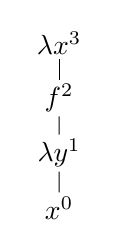
\begin{tikzpicture}[level distance=7mm,inner ysep=0.5mm]
 \node {$\lambda x^3$}
    child {
        node {$f^2$}
        child {
            node {$\lambda y^1$}
            child{
                node{$x^0$}
            }
        }
    };
\end{tikzpicture}
} \noindent \emph{Examples:} Consider the $\beta$-normal term
$\lambda x . f (\lambda y .x)$ where $x,y:o$ and $f:(o,o),o$. The
figure on the right represents the computation tree with the order
of each node in the exponent part. Since node $x$ of order $0$ is
not bound by the order 1 node $\lambda y$, $\tau(M)$ is not
incrementally-bound and by proposition
\ref{prop:Nher_incrbound_and_incrjustified} $\sem{\lambda x . f
(\lambda y .x)}$ is not P-incrementally-justified. Similarly we can
check that $\sem{f (\lambda y .x)}$ is not P-incrementally-justified
whereas $\sem{\lambda y. x}$ is. Also, for any higher-order variable
$x:A$ the computation tree $\tau(x)$ is incrementally-bound
therefore the projection strategies $\pi_i$ are
P-incrementally-justified. From these examples we observe that
application does not preserve P-incremental-justification ($\sem{f}$
and $\sem{\lambda y. x}$ are P-incrementally-justified whereas
$\sem{f (\lambda y .x)}$ is not).
\smallskip

These examples suggest that P-incremental-justification is not a
compositional property. In Chapter \ref{chap:pincrjust} we will
identify a sufficient condition for the composition of
two P-incrementally-justified strategies to be
P-incrementally-justified. \smallskip


Putting Corollary \ref{cor:Nher_incrbound_iff_incrjustified} and
Lemma \ref{lem:incrbound_iff_etanf_safe} together gives us a
game-semantic characterization of safe terms:
\begin{theorem}[Safety and P-incremental justification]
\label{thm:safeincrejust} Let $\Gamma \stentail M : A$ be a pure simply-typed term
(with no interpreted constants).
\begin{enumerate}[(i)]
\item If $\Gamma \stentail M : A$ is almost safe (and in particular if it is safe) then $\sem{\Gamma \stentail M : A}$
is P-incrementally justified.
\item If $\sem{\Gamma \stentail M : A}$ is
  P-incrementally justified then the eta-long normal form of the beta-normal form of $M$ is
almost safe, and safe if further $M$ is closed.
\end{enumerate}
\end{theorem}
In particular, a term has a P-incrementally justified denotation if and only
its eta-long beta-normal form is almost safe.

This result was first presented in TLCA2007, \cite[Theorem 3(ii)]{blumong:safelambdacalculus}.


\begin{corollary}[P's pointers are superfluous for safe terms]
\label{cor:safe_ptr_recoverable} Pointers emanating from P-moves in the game semantics of
safe terms are uniquely recoverable.
\end{corollary}
\begin{proof}
Let $M$ be a safe simply-typed term. Then the $\beta$-normal form of
$M$ is also safe, thus by lemma \ref{lem:incrbound_iff_etanf_safe}
(i), $\tau(\betanf{M})$ is incrementally-bound and by proposition
\ref{prop:Nher_incrbound_and_incrjustified}, $\sem{\Gamma \vdash
\betanf{M} :T}$ is a P-incrementally-justified strategy. By lemma
\ref{lem:incrjustified_pointers_uniqu_recover}, P's pointers in
$\sem{\Gamma \vdash \betanf{M} :T}$ are uniquely recoverable.
Finally, the soundness of the game model gives $\sem{\Gamma \vdash
M:T} = \sem{\Gamma \vdash \betanf{M} : T}$.
\end{proof}


\section{Safe PCF}
In this section will give a game-semantic characterization of Safe
PCF based on syntactical arguments.

We recall that the $\beta$-normal form of a \pcf\ term is the possibly infinite term obtained by reducing all the $\beta$-redexes. A $\beta$-normal form is therefore not necessarily normal with respect to the full system of rules of \pcf\ (\eg\ the term $\pcfcond\, 0\, M\, N$ is $\beta$-normal although it reduces in one step to $M$).

\subsubsection{Game characterization of safe terms}

In the context of the simply-typed lambda calculus, we have shown the
correspondence between safety and P-incremental justification (Theorem \ref{thm:safeincrejust}).
We will show (theorem \ref{}) that that the first part of the theorem
still holds for Safe \pcf. The second part, however, does not
hold anymore: Indeed, take the closed \pcf\ term $M = \lambda f x y. f
(\lambda z. \pcfcond (\pcfsucc\ x) y z )$ where $x,y,z:o$ and
$f:((o,o),o)$. $M$ is in normal form (conditional cannot be reduced
since the value of $x$ is undetermined). The $\eta$-long form of the
$\beta$-normal form of $M$ is therefore $M$ itself which is unsafe.
But clearly we have $\sem{M} = \sem{\lambda f x y. f (\lambda z.
z)}$, and since $\lambda f x y. f (\lambda z. z)$ is safe, by (i),
$\sem{M}$ is P-incrementally justified.

Such counter-example arises because the conditional operator of
\pcf\ permits us to construct terms in normal form that contain
``dead code'' {\it i.e.}~some subterm that will never be evaluated
for any value of M's parameters. In the example above, the dead code
consists of the subterm $y$. In general, if the dead code part of
the computation tree contains a variable that is not incrementally
bound then the resulting term will be unsafe even if the rest of the
tree is incrementally bound. In the example above, it was possible
to turn $M$ into the equivalent safe term $\lambda f x y. f (\lambda
z. z)$ by eliminating the dead code from $M$. In fact we can
generalise this method to any \pcf\ term with a P-incrementally
justified denotation.
\smallskip

Dead code elimination can be difficult to achieve in practice but it
is easy to define it formally: We say that a subterm $N$ occurring
in a context $C[-]$ in $M : (A_1, \ldots, A_n,o)$ is part of the
\defname{dead code} of $M$ if for any term $T_0$ of the form $M M_1
\ldots M_n$, any reduction sequence starting from $T_0$ does not
involve a reduction of the subterm $N$ {\it i.e.}~for any reduction
sequence $T_0 \redar T_1 \redar \ldots \redar T_k$, there is no
$j\in \{0.. k-1\}$ such that $T_j = C[N]$ and $T_{j+1} = C[N']$ for
some term $N'$.


Let $M$  be a \pcf\ term in $\eta$-nf. An occurrence of a variable
$x$ in $M$ is said to be a \defname{dead occurrence} if it occurs in
the dead code of $M$. In other words, it is a dead occurrence of $x$
if the corresponding node in the computation tree does not appear in
any traversal of $\travset(M)$. Equivalently, thanks to the
Correspondence Theorem, an occurrence of $x:B$ is dead if and only
if the initial move of the arena $\sem{B}$ does not appear in any
play of $\sem{M}$.


We define $M^*$ as the term obtained from $M$ after substituting all
subterms of the form  $x N_1 \dots N_k$ for some dead variable
occurrence $x:(B_1,\ldots, B_k, o)$ by the constant $0$. This
process is called \defname{dead variable elimination}. Note that if
$M$ is in $\eta\beta$-nf then so is $M^*$. We also write $\tau(M)^*$
to denote the equivalent transformation on the computation tree.
Since the computation tree is constructed from the $\eta$-nf of $M$,
we will use this notation even when $M$ is not in $\eta$-nf.



\begin{proposition}[Incremental-binding and P-incremental justification coincide] \
\label{prop:Nher_incrbound_and_incrjustified_pcf} Let $\Gamma \vdash
M : A$ be a PCF term in $\beta$-normal form.
\begin{enumerate}[(i)]
\item  If $\tau(\Gamma \vdash M : A)$ is incrementally-bound then $\sem{\Gamma \vdash M : A}$ is P-incrementally justified,
\item  if $\sem{\Gamma \vdash M : A}$ is P-incrementally justified
then $\tau(\Gamma \vdash M : A)^*$ is incrementally-bound.
\end{enumerate}
\end{proposition}
\begin{proof}
(i) The proof is exactly the same as in the simply typed lambda calculus case,
see \cite[Proposition 4.1.5(i)]{blumtransfer}.

\noindent (ii)
Take $\Gamma \vdash M : A$ a \pcf\ term in $\beta$-normal form denoted by $\sem{\Gamma \vdash M : A}$ P-incrementally justified. Let $r$ denote the root of $\tau(M)^*$.
Let $n$ be a node of $\tau(M)^*$ labelled by the variable $x$.
$\tau(M)^*$ is free from dead code therefore $n$ is not a dead occurrence of $x$ and there exists a traversal of $\tau(M)^*$ of the form $t \cdot x$.

\pcf\ constants are of order $1$ at most therefore they cannot
hereditarily justify a variable node, thus $x$ is necessarily
hereditarily justified by the only occurrence $r$ of the root of the
computation tree.

By considering $t\cdot x$ as a traversal of $\tau(M)$,  the
correspondence theorem gives $\varphi((t \cdot x) \filter r) =
\varphi((t \filter r) \cdot x) \in \sem{M}$. Since $\sem{M}$ is
P-incrementally justified, $\varphi(x)$ must point to the last
O-move in $\pview{\varphi(t \filter r)}$ with order strictly greater
than $\ord{\varphi(x)}$. Consequently $x$ points to the last node in
$\pview{t \filter r} \filter N^{\lambda}$ with order strictly
greater than $\ord{x}$. We have:
\begin{align*}
\pview{t \filter r} &= \pview{t} \filter N^{r \vdash} & (\mbox{by Lemma \ref{lem:betanf_wellbehavedconst_trav_pview_red}}) \\
& = [r,x[ \ \filter N^{r \vdash} & (\mbox{by Prop.\ \ref{prop:pviewtrav_is_path}})
\end{align*}
\notetoself{review use of Lemma
\ref{lem:betanf_wellbehavedconst_trav_pview_red}}

Since $M$ is in $\beta$-nf, the set of nodes not hereditarily
enabled by $r$ is exactly the set of nodes hereditarily enabled by
$N_{\Sigma}$ thus $[r,x[ \ \filter N^{r \vdash} = [r,x[\ \setminus\
N^{\filter \Sigma}$. Moreover \pcf\ constants are of order $1$ at
most therefore $N^{\filter \Sigma} = N_{\Sigma} \union N^c_{\Sigma}$
where $N^c_{\Sigma}$ is the set of children nodes of $N_{\Sigma}$.
Thus $\pview{t \filter r} \filter N^{\lambda} = ([r,x[\ \setminus\
N_{\Sigma} \setminus N^c_{\Sigma} ) \filter N^{\lambda} = ([r,x[\
\setminus\  N^c_{\Sigma} )  \filter N^{\lambda}$, and since
$N^c_{\Sigma}$ is constituted of order $0$ lambda-nodes only, $x$
must point to the last node in $[r,x[ \filter N^{\lambda}$ with
order strictly greater than $\ord{x}$.

Hence if $x$ is a bound variable node then it is bound by the
last $\lambda$-node in $[r,x[$ with order strictly greater than
$\ord{x}$ and if $x$ is a free variable then it points to $r$ and
therefore all the $\lambda$-node in $]r,x[$ have order smaller than
$\ord{x}$. Thus $\tau(M)^*$ is incrementally-bound.
\end{proof}

The counterpart of Lemma 4.1.6 from
\cite{blumtransfer} can be stated as follows in the context of PCF:
\begin{lemma}[Almost safety and incrementally-binding]
\label{lem:incrbound_iff_etanf_safe_pcf} Let $\Gamma \vdash M : A$
be a PCF term.
\begin{itemize}
\item[(i)] If $\Gamma \vdash M : A$ is almost safe then $\tau(\Gamma \vdash M : A)$ is incrementally-bound ;
\item[(ii)] conversely, if $\tau(\Gamma \vdash M : A)$ is incrementally-bound then the $\eta$-normal form of $\Gamma \vdash M : A$ is almost safe if $M$ is open and safe if $M$ is closed.
\end{itemize}
\end{lemma}
The proof can be obtained by adapting the proof
of Lemma 4.1.6 from \cite{blumtransfer}.

A difficulty arises because of the presence of the Y combinator :
computation trees of \pcf\ terms are potentially infinite. Despite
this particularity, lemma \ref{lem:incrbound_iff_etanf_safe} still
holds in the \pcf\ setting:

\begin{lemma} \label{lem:pcf_safe_imp_incrbound} The computation tree of a Safe PCF term is incrementally-bound.
\end{lemma}
\begin{proof}
\notetoself{adapt this proof to almost safe terms}
(i) Let $M$ be a safe PCF term and  $i$ denote the number of occurrences of the Y combinator in $M$.
We first prove by induction on $i$ that $M_k$ is safe for any $k\in
\omega$. \emph{Base case:} $i=0$ then $M_k = M$. \emph{Step case:}
$i>0$. Let $Y_A N$ be a subterm of $M$. Since $M$ is safe, $N$ is
also safe. The number of occurrences of the Y combinator in $N$ is
smaller than $i$ therefore by the induction hypothesis $N_k$ is
safe. Consequently the term $Y_A^k N_k = \underbrace{N_k ( \ldots (
N_k}_{k \mbox{ times}} \Omega ) \ldots )$ is also safe and by
compositionality so is $M_k$.

Clearly, lemma \ref{lem:incrbound_iff_etanf_safe}(i) remains
valid for infinite $\pcf_1$ terms (the subterms of the form $\Omega$
are just represented by the constant $\bot$ in the computation
tree), thus since $M_k$ is a safe $\pcf_1$ term, $\tau(M_k)$ is
incrementally-bound. Now let $z$ be a variable node in $\tau(M) =
\Union_{k\in\omega} \tau(M_k)$. There exists $k\in \omega$ such that
$z$ belongs to $\tau(M_k) \sqsubseteq \tau(M)$. If we write $r_k$ to
denote the root of the tree $\tau(M_k)$ then the path $[r_k,z]$ in
$\tau(M_k)$ is equal to the path $[r,z]$ in $\tau(M)$. Hence, since
the node $z$ is incrementally-bound in $\tau(M_k)$, it is also
incrementally-bound in $\tau(M)$.
\end{proof}




\begin{theorem}[Almost safety and P-incremental justification]
\label{thm:almostsafeincrejust_pcf} Let $\Gamma \vdash M : A$ be a PCF term. Then:
\begin{enumerate}[(i)]
\item If $\Gamma \vdash M : A$ is almost safe then $\sem{\Gamma \vdash M : A}$ is P-incrementally justified.
\item If $\sem{\Gamma \vdash M : A}$ is
  P-incrementally justified then $\etalnf{\betanf{M}}^*$ is
  almost safe  if $M$ is open, and safe if $M$ is closed.
\end{enumerate}
\end{theorem}

\begin{proof}
\noindent(i)
A proof of this is given in the proof of Theorem 4.2.10 in \cite{blumtransfer}.

\noindent(ii) Suppose $M$ is a \pcf\ term with a P-incrementally
justified strategy denotation. By Proposition
\ref{prop:Nher_incrbound_and_incrjustified_pcf}(ii),
$\tau(\betanf{M})^* = \tau(\etalnf{\betanf{M}}^*)$ is
incrementally-bound. If $M$ is closed then so is
$\etalnf{\betanf{M}}^*$ therefore by Lemma
\ref{lem:incrbound_iff_etanf_safe_pcf},
$\etalnf{\etalnf{\betanf{M}}^*} = \etalnf{\betanf{M}}^*$ is safe. If
$M$ is open then so is $\etalnf{\betanf{M}}^*$ and by Lemma
\ref{lem:incrbound_iff_etanf_safe_pcf},
$\etalnf{\etalnf{\betanf{M}}^*} = \etalnf{\betanf{M}}^*$ is
almost safe.
\end{proof}

\begin{theorem}
Safe PCF terms are denoted by P-incrementally-justified strategies.
\end{theorem}
\begin{proof}
Let $M^{\infty}$ be the $\beta$-normal form of $M$ (i.e. the possibly infinite term obtained by reducing all the $\beta$-redexes in $M$). By lemma \ref{lem:ia_safety_preserved}, safety is preserved by small-step reduction therefore, by lemma \ref{lem:pcf_safe_imp_incrbound}, if $M$ is a \pcf\ term then $\tau(M^{\infty})$ is also
incrementally-bound.

Since \pcf\ constant rules are well-behaved (by Lemma
\ref{lem:sigma_order1_are_wellbehaved}), the result from Lemma
\ref{lem:betanf_wellbehavedconst_trav_pview_red} is also true for
Safe \pcf. Thus proposition
\ref{prop:Nher_incrbound_and_incrjustified}(i) remains valid for the
infinite computation trees of \pcf: infinite terms in $\beta$-nf
with an incrementally-bound computation tree are denoted by
P-incrementally-justified strategies. Consequently,
$\sem{M^{\infty}}$ is P-incrementally-justified. By soundness of the
game denotation, $\sem{M^{\infty}} = \sem{M}$, thus $\sem{M}$ is
P-incrementally-justified.
\end{proof}

Consequently, P-pointers are superfluous in the game denotation of safe \pcf\ terms {\it i.e.} pointers emanating from P-moves are uniquely recoverable.

We write \pcf' to denote the language obtained by extending \pcf\
with the $\pcfcase_k$ construct (see \cite{Abr02}).
The $\pcfcase_k$ construct is the obvious generalisation of the
conditional operator \pcfcond\ to $k$ branches instead of $2$. All the results obtained so far concerning Safe \pcf\ (including those
cited from \cite{blumtransfer}) can clearly be transposed to \pcf'.

\subsubsection{Definability result}

The previous theorem leads to the following definability result for safe \pcf':
\begin{proposition}[Definability for safe \pcf' terms]
\label{prop:safetydefinability} Let $\overline{A}=(A_1,\ldots, A_i)$
and $B =(B_1, \ldots, B_l,o)$ be two PCF types for some $i,l\geq 0$
and $\sigma$ be a well-bracketed innocent P-i.j.\ strategy with
finite view function defined on the game $!A_1 \otimes \ldots
\otimes !A_i \lingamear (!B_1 \lingamear \ldots \lingamear !B_l
\lingamear o) $. There exists an \emph{almost safe} PCF' term
$\overline{x} : \overline{A} \vdash M : B$ in $\eta$-long normal
form such that:
$$ \sem{\overline{x} : \overline{A} \vdash M_\sigma : B} = \sigma $$
and a safe closed PCF' term $\vdash_s M'_\sigma : (\overline{A},B)$ in $\eta$-long normal form such that:
$$ \sem{\vdash M'_\sigma : (\overline{A},B)} \cong \sigma \ .$$
\end{proposition}
\begin{proof}
By the standard definability result for PCF', there is a term
$\overline{x} : \overline{A} \vdash N : B$ such that
$\sem{\overline{x} :\overline{A} \vdash N : B} = \sigma$. Take
$M_\sigma$ to be $\etalnf{\betanf{N}}^* $. We have
$\sem{\overline{x} : \overline{A} \vdash M_\sigma : B} =
\sem{\overline{x} :\overline{A} \vdash N : B} = \sigma$ and by
Theorem  \ref{thm:almostsafeincrejust_pcf}(ii), $M_\sigma$ is
almost safe. For the second part we just need to take $M'_\sigma =
\lambda \overline{x}. M_\sigma$.
\end{proof}


\subsubsection{Compositionality of P-i.j.\ strategies (syntactic
argument)}


We have already shown in Sec. \ref{sec:closedpij} that under certain
conditions, P-i.j.\ strategies compose. Here we will obtain a
slightly weaker version of this result using a much simpler argument
which exploits the definability result from the previous section.


 Let $\overline{A} = (A_1, \ldots, A_i)$, $B = (B_1, \ldots,
B_l,o)$ and $C=(C_1,\ldots,C_k,o)$ be three PCF types for some
$i\geq 1,l,k\geq 0$. Let $f:\ !A_1 \otimes \ldots \otimes !A_i
\lingamear B$ and $g:\ !B\lingamear C$ be two innocent
well-bracketed and P-incrementally justified strategies with finite
view function. We would like to find under which conditions the
composition $f\fatcompos g$ is also P-incrementally justified.

By the definability result, there are two closed safe terms (in $\eta$-nf) $\vdash M_f :(\overline{A},B)$  and $\vdash M_g :B \typear C$ such that $\sem{M_f} = f$
and $\sem{M_f} = g$.
We define the term $M_{f\fatcompos g} = \lambda \overline{x} . M_g (M_f \overline{x})$ for some fresh variables $\overline{x} : \overline{A}$. Clearly we have $\sem{M_{f\fatcompos g}} = \sem{M_f} \fatcompos \sem{M_g} = f\fatcompos g$.

\paragraph{Sufficient conditions}

By Theorem \ref{thm:almostsafeincrejust_pcf}, we know that
$f\fatcompos g$ is P-incrementally justified just when
$\etalnf{\betanf{M_{f\fatcompos g}}}^*$ is safe. We will now exploit
this fact to extract a sufficient condition on the types $A$ and $B$
for the composition of $f$ and $g$ to be P-incrementally justified.

The term $M_f$ and $M_g$, being in $\eta$-nf, are of the following forms:
\begin{eqnarray*}
\vdash M_f &=& \lambda x_1^{A_1} \ldots x_i^{A_i} \varphi_1^{B_1} \ldots \varphi_l^{B_l} . N_f^o\\
\vdash  M_g &=& \lambda y^{ (B_1, \ldots, B_l,o)} \phi_1^{C_1} \ldots \phi_k^{C_k} . N_g^o
\end{eqnarray*}
for some distinct variables $x_1, \ldots, x_i$, $y$, $\varphi_1, \dots \varphi_l$, $\phi_1, \dots \phi_k$  and $\eta$-normal terms $N_f$ and $N_g$:
\begin{eqnarray*}
x_1:A, \ldots, x_i:A_i, \varphi_1:B_1, \dots, \varphi_l:B_l &\vdash& N_f :o \\
y: (B_1, \ldots, B_l,o), \phi_1:C_1, \dots, \phi_l:C_l &\vdash& N_g :o
\end{eqnarray*}



The fact that $M_f$ and $M_g$ are safe does not imply that $M_{f\fatcompos g}$ is: take $M_f = \lambda x^o z^o.x$ and $M_g = \lambda y^{(o,o)} . y a$ for some constant $a\in \Sigma$, then $\lambda x:A . M_g (M_f x) = \lambda x . (\lambda y . y a) ( \underline{(\lambda x z.x) x} )$ is unsafe because of the underlined subterm. However we have:
\begin{align*}
f\fatcompos g &= \sem{\lambda \overline{x} . M_g (M_f  \overline{x})} \\
 &= \sem{\lambda \overline{x} . (\lambda \phi_1\ldots \phi_k . N_g) [(M_f \overline{x}) / y]} \\
&= \sem{\lambda \overline{x} \phi_1 \dots \phi_k. N_g [(M_f  \overline{x}) / y]}
& \mbox{(the $x_j$'s and $\phi_j$'s are disjoint)}.
\end{align*}

We now concentrate on the term  $\lambda \overline{x} \phi_1 \dots
\phi_k. N_g [(M_f  \overline{x}) / y]$ and try to find a sufficient
condition guaranteeing its safety.

\subparagraph{A sufficient condition}
\begin{lemma}
Suppose that $\Gamma,y:B \vdash M$ is a safe term in $\eta$-nf and $\Gamma \vdash R : B$ is an almost safe application. Let $N$ denote the set of nodes of the computation tree $\tau(M)$. We have:
\begin{align*}
\Gamma \vdash M[R/y] :A \mbox{ safe }
\iff&  \forall x \in fv(R) . \\
    & \forall n_y \in N_{\sf fv} \mbox{ labelled $y$}.
      \forall m \in N_{\lambda} \inter ]r,n_y] : \ord{m} \leq \ord{x}
\end{align*}
\end{lemma}
\begin{proof}
Since $M$ is in $\eta$-nf, all the application to the variable $y$ are total (i.e.~of the form $y P_1 \ldots P_l :o$). Hence after substituting the safe term $N$ for $y$ in $M$, the only possible cause of unsafety is when
some variable free in $N$ becomes not safely bound in $\tau(M)$.
\end{proof}

Applying this lemma with $R= M_f \overline{x}$ gives us a sufficient
condition -- the right-hand side of the equivalence -- for $\lambda
x \phi_1 \dots \phi_k. N_g [(M_f \overline{x}) / y]$ to be safe, and
hence for $f\fatcompos g$ to be P-incrementally justified. Of course
it is not a necessary condition since $N_g[(M_f \overline{x}) /y]$
can be unsafe while its eta-beta normal form is safe.

\subparagraph{A simpler sufficient condition}
\begin{lemma}
If $y:B, \Sigma \vdash N : T$ and $\vdash M : (\overline{A}, B)$
are safe terms with $\ord{A_i} \geq \ord{B}$ for all $i\in 1..n$
then $\overline{x}:\overline{A}, \Sigma \vdash N[(M \overline{x})/y] :T$ is also safe.
\end{lemma}
\begin{proof}
Since $\ord{x_i} = \ord{A_i} \geq \ord{B} = \ord{M \overline{x}}$, we can use the application
rule of the safe lambda calculus to form the safe term $\overline{x}:\overline{A} \vdash M \overline{x}$.
Using the substitution lemma we have that $N[(M \overline{x})/y]$ is safe.
\end{proof}

Hence we obtain the following sufficient condition for $f\fatcompos
g$ to be P-incrementally justified:
$$\ord{A_i}\geq\ord{B} \mbox{ for all } 1 \leq i \leq n$$


Indeed the lemma gives that $\vdash \lambda \overline{x} \phi_1
\dots \phi_k. N_g [(M_f \overline{x}) / y]$ is safe and therefore
its denotation $\sem{\vdash \lambda \overline{x} \phi_1 \dots
\phi_k. N_g [(M_f \overline{x}) / y]} = f\fatcompos g$ is
P-incrementally justified.

Note that this condition is not necessary: Take $A=o$, $B=(o,o)$,
$C=(o,o)$ and consider the two safe terms $M_f = \lambda x^A u^o.u$
and $M_g = \lambda y^B . y a$ for  some constant $a:o$. Then we have
$M_{f\fatcompos g} = \lambda x . a$ which is safe hence $f\fatcompos
g$ is P-incrementally justified although $\ord{A} < \ord{B}$.

\begin{remark}
This result corroborates what we already know about compositionality
of P-i.j.\ strategies (see Sec. \ref{sec:closedpij}). Indeed, the
condition given hereinbefore implies that the strategy $f$ is
\emph{closed} P-i.j.\ (the $A_i$s are prime because we are working
with PCF types) and therefore by Prop.\ \ref{prop:closedpijcompose},
$f \fatcompos g$ must also be P-i.j.
\end{remark}




\paragraph{Counter-example: two P-i.j.\ strategies whose composition is not
P-i.j.}

We now give counter-example to show that P-i.j.\ strategies do not
compose in general.

\subparagraph{First attempt}

Take the types $A=o$, $B=(o,o)$, $C=o$, the variables
$x,u,v:o$, $y:B$ and $\varphi:((o,o),o)$ and $\Sigma$-constant $a:o$.
Consider the two safe terms $\vdash_s  M_f = \lambda xv.x : A\typear B$ and $\vdash_s M_g = \lambda y . \varphi (\lambda u . y a) : B\typear C$.
The $\eta\beta$-nf of $M_{f\fatcompos g}$ is $\vdash \lambda x . \varphi (\underline{\lambda u . x})$ which is unsafe because of the underlined term. It is then tempting to use
Theorem \ref{thm:safeincrejust}(ii) to conclude that
$\sem{M_{f\fatcompos g}}$ is not P-incrementally justified. However this theorem cannot be used here because $M_g$ contains an order $2$ constants ($\varphi$) therefore
$M_{f\fatcompos g}$ is not a valid simply typed $\lambda$-term (nor a \pcf-term).

\subparagraph{Second attempt} The previous example can be easily
changed into a working counter-example: we just need to elevate
$\varphi$ from the status of constant to variable.

Take $A=o$, $B=(o,o)$, $C=(((o,o),o),o)$, the variables
$x,u,v:o$, $y:B$ and $\varphi:((o,o),o)$ and the $\Sigma$-constant $a:o$. Consider the two safe terms $\vdash_s  M_f = \lambda xv.x : A\typear B$ and  $\vdash_s M_g = \lambda y \varphi. \varphi (\lambda u . y a) : B\typear C$.
The $\eta\beta$-nf of $M_{f\fatcompos g}$ is $\vdash \lambda x \varphi. \varphi (\underline{\lambda u . x})$ which is unsafe because of the underlined term, thus by Theorem \ref{thm:safeincrejust}(ii), $\sem{M_{f\fatcompos g}}=\sem{M_f} \fatcompos
\sem{M_g}$ is not P-incrementally justified. The following diagram illustrates a play that is not P-i.j.:

\begin{center}
\begin{tikzpicture}[style={anchor=base}]
\matrix (m) [matrix of math nodes]
{
    \ &   & \ & \ & \ & \ &  & &\  &  & & & \\
    o & \stackrel{\sigcol{\sem{M_f}}}\longrightarrow & (o, & o) & \stackrel{\mucol{\sem{M_g}}}\longrightarrow & (((o, &o),& o),& o) \\ \\
    &&&&&&&&\node(n0){\lambda x \varphi \omove  \mucol {\lambda y \varphi}};\\[3mm]
    &&&&&&&\node(n1){\varphi  \pmove \mucol \varphi};\\[3mm]
    &&&&&&\node(n2){\lambda u \omove  \mucol {\lambda u}}; \\[3mm]
    &&&  \node(n3){ \sigcol {\lambda x v} \opmove \mucol y}; \\[3mm]
    \node(n4){x \pmove \sigcol x}; \\
};
\draw [-,thick] (m-1-1.south west) -- (m-1-1.south east) node [above,midway] {A};
\draw [-,thick] (m-1-3.south west) -- (m-1-4.south east) node [above,midway] {B};
\draw [-,thick] (m-1-6.south west) -- (m-1-9.south east) node [above,midway] {C};
\path (n4) edge[tableptr] (n0);
\path (n2) edge[tableptr,\mucolor] (n1);
\path (n1) edge[tableptr,\mucolor] (n0);
\path (n3) edge[tableptr,\mucolor] (n0);
\path (n4) edge[tableptr,\sigcolor] (n3);
\end{tikzpicture}
\end{center}


\subparagraph{Another counter-example with $\ord{B} = \ord{C}$.}

Let $A=o$, $B=C=(((o,o),o),o)$ and let $x:A$, $y:B$, $u:o$, $v,\varphi:((o,o),o)$
and $g:(o,o)$ be variables and  $a:o$ be a $\Sigma$-constant. Take the two safe terms $\vdash  M_f = \lambda x v.x$ and $\vdash M_g = \lambda y \varphi. \varphi (\lambda u . y (\lambda g. a))$.
The $\eta\beta$-nf of $M_{f\fatcompos g}$ is $\vdash \lambda x \varphi. \varphi (\underline{\lambda u . x})$ which is unsafe because of the underlined term, so
$f\fatcompos g$ is not P-incrementally justified.


\section{Safe Idealized Algol}
\notetoself{Section to be written...}

In this section we show how the syntactic argument used to give the game characterization of the safe lambda calculus can be adapted to the setting of Safe \ialgol.
The type system for Safe \ialgol\ is given in section \ref{subsec:safeia_rules}.

Ultimately this allows us to show that the pointers in the game denotation of safe IA terms can be recovered uniquely. Such result has potential applications in algorithmic game semantics: using ideas from \cite{ghicamccusker00},
it may be possible to give a characterisation of the game semantics
of some higher-order fragments of safe \ialgol\ using extended
regular expressions, which would subsequently lead to a decision procedure for
observational equivalence of program from the considered fragment.
\notetoself{prove this conjecture!}

\notetoself{ Overview of the argument:

Clearly, the computation hypertree of a safe term is incrementally-bound.
By using the correspondence between traversals and plays, it is easy
to prove that incrementally-bound computation trees are denoted by
P-incrementally-justified strategies. Consequently, by lemma
\ref{lem:incrjustified_pointers_uniqu_recover}, P's pointers are superfluous in the
game semantics of safe \ialgol\ terms.

Since the game denotation of an \ialgol\ term is fully determined by
the set of complete plays, this pointer economy suggests that the
game denotation of a safe \ialgol\ can be represented in a compact
way. This raises the question of the decidability of observational
equivalence for safe \ialgol.
} 